\chapter{Einleitung}\label{sec:1_einleitung}
In diesem Kapitel wird die wissenschaftliche und praktische Motivation dieser Thesis dargelegt. Des Weiteren, wird der Projekt-Kontext dieser Arbeit erläutert um Hintergrund, Ziel und Abgrenzung dieser Arbeit besser verständlich zu machen. Zuletzt wird ein Überblick über die restlichen Kapitel dieser Thesis gegeben.


\section{Motivation}\label{sec:1_motivation}
\ac{Ubicomp}, die Allgegenwart der virtuellen Welt in der Realität wird von vielen Designern erforscht \cite{Kuniavsky.2010}. Um Interaktion mit Systemen zu ermöglichen, ohne explizite \acp{UI} zu verwenden, werden neue Konzepte und Technologien benötigt. Seit Beginn des 21. Jahrhunderts hat sich \ac{IoT} als Schlüsselparadigma herauskristallisiert, um virtuelle und reale Welt verschmelzen zu lassen \cite{Gubbi.2013}. \ac{IoT}-Produkte reichen von Glühbirnen\footnote{\url{http://www.meethue.com}}, die auf ihre Umgebung reagieren, bis hin zu intelligentem Besteck\footnote{\url{https://www.hapi.com/}}, welches das Essverhalten von Nutzern aufnimmt. Durch das Ausnutzen der digitalen Welt, haben sich Produkte auf dem Markt etabliert, welche die \ac{UX} ihrer analogen Vorgänger erweitern.

Obwohl die theoretischen Vorteile von intelligenten Objekten zahlreich sind, mangelt es oftmals noch an ihren praktischen Umsetzungen -- vor allem im Bereich der \ac{UX} \cite{Resnick.2013}. Diesem Umstand liegt die Tatsache zu Grunde, dass Produktentwicklung und Forschung im Bereich der \ac{IoT}, Designer und Wissenschaftler vor neue Herausforderungen stellt. Um die Effektivität neuer \ac{IoT}-Konzepte empirisch validieren zu können \cite{Robinson.2018}, benötigt es Prototypen, die diese Konzepte umsetzen. 

Das Entwickeln von \ac{IoT}-Prototypen, verlangt von Forschern und Designern, dass sie sich eine große Menge an technischem Fachwissen aneignen. Dieses Fachwissen lässt sich in zwei Teile auftrennen: 

\textbf{Erstens}, hardwarenahes Wissen (bspw. Elektrotechnik, Signalverarbeitung und Netzwerktechnik) um Komponenten und Infrastruktur der Prototypen bauen zu können. Diesem Problem nimmt sich \cite{weckbach2018cblocks} mit dem Werkzeug \acp{cBlock} an. 

\textbf{Zweitens} und Motivation dieser Thesis, ist das benötigte Wissen im Bereich des Software-Engineering und der Programmierung. \textit{Smart Devices} und \textit{connected Products} können nur so intelligent sein, wie sie programmiert werden. Aus diesem Grund, muss sich der Designer intensiv mit der Komplexität der Programmierung als Ganzes und den Besonderheiten von hardwarenaher Programmierung auseinandersetzen. Diese zusätzliche Arbeitsbelastung ist nur bedingt zumutbar und bei der Erforschung von \ac{IoT}-Konzepten nicht zielführend.

Das Aneignen dieses Wissens stellt eine Barriere für ''Nicht-Experten'' wie Designer dar. Gleichzeitig besitzen diese ''Nicht-Experten'' allerdings essentielles Wissen im Bereich der \ac{UX}. Es müssen daher Wege gefunden werden, diese Hürden zu nehmen oder zumindest so zu senken, dass eine iterativen Entwicklung von \ac{IoT}-Prototypen ohne tiefgründiges Fachwissen möglich ist. 

\section{Kontext}\label{sec:1_kontext}
Diese Thesis wird im Zusammenhang eines zweijährigen Forschungsprojekts geschrieben, dessen Ziel es ist, geeignete Werkzeuge zu erforschen, welche die Kommunikation zwischen Produkt-Entwicklung/Design und Kunden durch den Einsatz von Prototyp-getriebener Entwicklung zu verbessern. Im Zuge dieses Projekts werden verschieden Prozesse, Software und Hardware entwickelt. Diese Komponenten sollen kleinen und mittelständischen Unternehmen bei der Erstellung von Prototypen im Bereich \ac{IoT}, Webtechnologien und Virtual Reality/Augmented Reality helfen.

\begin{figure}[ht]
    \centering
    \begin{subfigure}[b]{0.3\textwidth}
        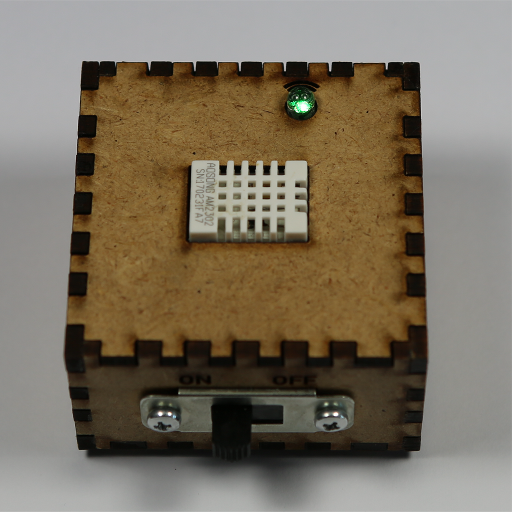
\includegraphics[width=1\linewidth]{bilder/chapter1/DHT22.png}
        \caption{}
        \label{fig:gull}
    \end{subfigure}
    \quad
    \begin{subfigure}[b]{0.3\textwidth}
        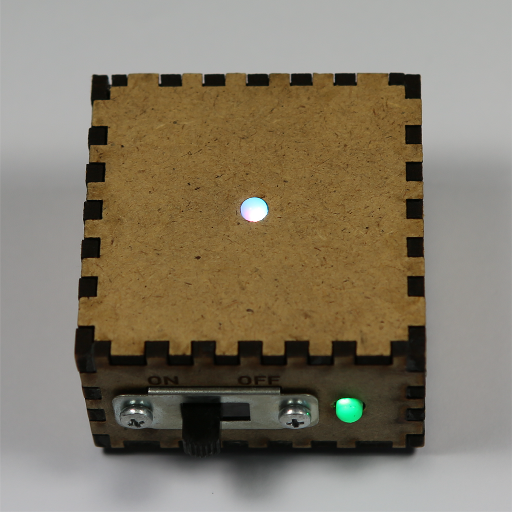
\includegraphics[width=1\linewidth]{bilder/chapter1/LED.png}
        \caption{}
        \label{fig:tiger}
    \end{subfigure}
    \quad
    \begin{subfigure}[b]{0.3\textwidth}
        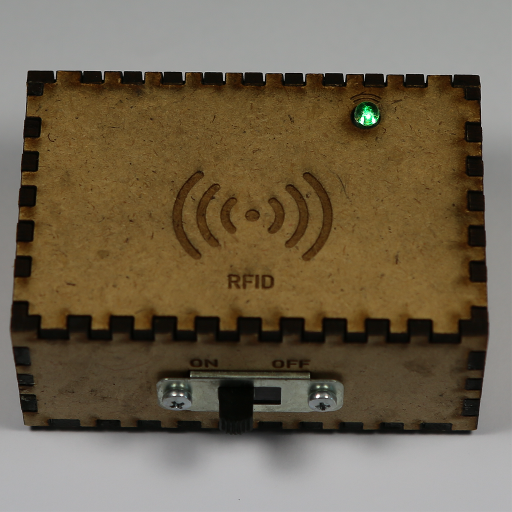
\includegraphics[width=1\linewidth]{bilder/chapter1/RFID.png}
        \caption{}
        \label{fig:mouse}
    \end{subfigure}
    \caption{Typische \acp{cBlock}. Hier bestehend aus drei unterschiedlichen Blöcken: Temperatur-Sensor (a),  LED-Aktor (b) und RFID-Sensor (c)}
    \label{fig:cblockfoto}
\end{figure}

Im Zuge dessen, wurde die Hardwareplattform \acp{cBlock} entwickelt. \acp{cBlock} ist ein \textit{open-source} Bausteinsystem zur Unterstützung von Designern beim Prototyping-Prozess von \ac{IoT} Produkten. Ein jeder Baustein abstrahiert verschiedenen Sensoren oder Aktoren und versucht dadurch, die Komplexität von hardwarenahen Entwicklungsaufgaben (beispielsweise Verdrahtung der Komponenten, Kommunikation zwischen Sensoren und Aktuatoren, Wählen von Protokollen) zu reduzieren. Das wichtigste Ziel von \acp{cBlock} ist allerdings nicht nur eine Aufwandsreduzierung auf Hardware-Ebene durchzuführen, sondern auch die Eintrittsbarriere für die Programmierung der Logik herunter zusetzen. Dadurch soll der technische Arbeitsaufwand von Designern so reduziert werden, dass sie sich darauf fokussieren können, neue \ac{IoT}-Erfahrungen zu erproben.

\section{Zielsetzung}\label{sec:1_zielsetzung}
Das \textbf{Ziel} dieser Arbeit darin, dem \textit{End-User} (d.h. dem Designer) bei der Erstellung von Programmlogik, welche die \ac{cBlock} steuern, zu unterstützen. Hierfür wird eine \ac{EUD}-Plattform konzipiert und evaluiert, welche auf die Anforderungen der Domäne des \ac{IoT} sowie den Anforderungen der Domänenexperten, gerecht wird. Dieses \ac{EUD}-Werkzeug, genannt \textit{flowws}, soll es Designern ermöglichen zusammen mit der \acp{cBlock}-Hardware, funktionale Prototypen zu gestalten.

Folgende \textbf{Forschungsfragen} sollen beantwortet werden:

\begin{itemize}
    \item \textbf{\#1 -- Analyse \& Anforderung} Wie schon im vorangeschrittenen Kapitel beschrieben, ist das Projekt durch spezielle Rahmenbedingungen bzgl. Prozessen und Stakeholdern gekennzeichnet. Deshalb die Frage:
    \begin{itemize}
        \item Welche fundamentalen Probleme müssen \ac{EUD}-Werkzeuge in der \ac{IoT}-Domäne überwinden?
        \item Welche Anforderungen stellt die \ac{IoT} und die involvierten Stakeholder an ein \ac{EUD}-Werkzeug?
    \end{itemize}
        \item \textbf{\#2 -- Konzeption} Die Analyse der Problemdomäne resultiert in den Anforderungen an das Konzept. 
    \begin{itemize}
        \item Wie können die Eigenheiten der Anwendungsdomäne in ein \ac{EUD}-Konzept übertragen werden?
    \end{itemize}
    \item \textbf{\#3 -- Evaluation} Im Anschluss zur Anforderungserhebung und Erarbeitung eines Konzepts eines \ac{EUD}-Werkzeuges soll die Wirksamkeit der Entscheidungen diskutiert und folgende Fragen beantwortet werden: 
    \begin{itemize}
        \item Was sind die Vorteile des erarbeiteten Konzepts und inwiefern lassen sich die Erkenntnisse auf zukünftige Projekte in diesem Themenbereich übertragen?
    \end{itemize}
\end{itemize}

\paragraph{Abgrenzung} Es ist nicht Ziel dieser Arbeit eine vollständige \ac{EUD} für einen Produktiveinsatz (bspw. in Form einer Turing-Vollständigen \ac{DSL}) zu konzipieren, sondern vielmehr geeignete Metaphern finden und \ac{UI}-Ansätze zu konzipieren und zu evaluieren, um einen besseren Einblick für zukünftige Projekte im Bereich des \ac{IoT}-Prototyping zu erhalten. Des Weiteren, grenzt sich diese Arbeit von hardware-technisch ähnlichen Systemen wie bspw. eBlocks \cite{Phalke.2010} ab, indem der Anwendungsfokus nicht auf Werkzeug zur Bildung im Bereich Software Engineering oder \ac{IoT} gelegt wird. Vielmehr handelt es sich bei flowws um ein Entwicklungswerkezug, welches aktiv zur Erprobung und Entwicklung von \ac{IoT}-Prototypen dienen soll.

\section{Aufbau der Arbeit}\label{sec:1_aufbau}
\begin{itemize}
    \item \textbf{Kapitel 1 Einleitung:} Eine Übersicht über das Thema und dem Kontext indem sie entstanden ist.
    \item \textbf{Kapitel 2 Grundlagen und State-of-the-Art:} In diesem Kapitel, werden die fundamentalen Wissensbausteine der \ac{IoT}- und \ac{EUD}-Domäne diskutiert. Zusätzlich werden bestehende \acp{EUD}-Systeme mit vergleichbarem Fokus diskutiert.
    \item \textbf{Kapitel 3 Anforderungen:} In diesem Abschnitt, werden Probleme von bestehenden \acp{EUD}-Systemen und die Stakeholder anhand einer Persona analysiert. Daraus abgeleitet, entstehen Vision und Ziele für das \ac{EUD}-Werkzeug, welche wiederum in Szenarios und Anforderungen transformiert werden.
    \item \textbf{Kapitel 4 Konzeption:} Das \ac{EUD}-Werkzeug flowws wird in diesem Kapitel konzipiert und die getroffen Designentscheidungen werden rationalisiert.
    \item \textbf{Kapitel 5 Evaluation:} Das Konzeptmodell von flowws wird durch Nutzertests auf seine Verständlichkeit überprüft.
    \item \textbf{Kapitel 6 Diskussion:} Zum Schluss werden die erarbeiteten Ergebnisse zusammengefasst, bewertet und ein Ausblick für zukünftige Arbeiten gegeben.
\end{itemize}